\documentclass[12pt,a4paper,fleqn]{article}
\usepackage[utf8]{inputenc}
\usepackage[russian]{babel}
\usepackage{amssymb, amsmath, multicol}
\usepackage{enumitem}
\usepackage{lipsum}
\usepackage{euler}
\oddsidemargin=-15.4mm
\textwidth=190mm
\headheight=-32.4mm
\textheight=277mm
\parindent=0pt
\parskip=8pt
\pagestyle{empty}
\usepackage{graphicx}
\title{\textbf{\LARGE{Исследовательская работа по теме:\\Исследование функции дифференциальными методами}}}
\author{Известный гражданин}
\date{November 2022}
\addt\captionsrussian{\def\refname{Список литературы}}\begin{document}
\maketitle
\newpage\newpage \textbf{\LARGE{Глава I. Функция}}

\begin{center}
$y = $$log(x)$

\end{center}
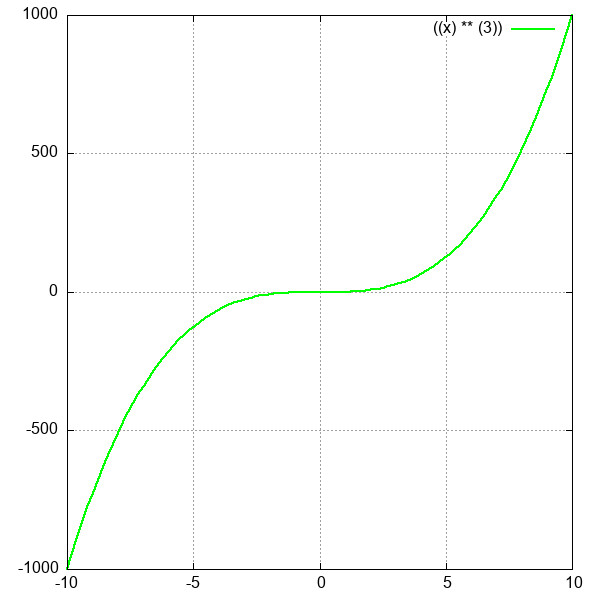
\includegraphics{GraphicDumps/plot.jpg}\newpage \textbf{\LARGE{Глава II. Визуальный анализ функции}}

Обоснование этого перехода было забанено редактурой

\begin{center}
$y = $$log(x)$

\end{center}
\newpage \textbf{\LARGE{Глава III. Дифференцирование}}

Ну вот как этот матан тебе в жизни пригодится?

\begin{center}
 ($x)'
  = 1$\end{center}
Телец в козероге, поэтому

\begin{center}
 ($log(x))'
  = (\frac{1}{x} \cdot 1)$\end{center}
\newpage \textbf{\LARGE{Глава IV.Упрощение выражения}}

Любовь - это верить в его выводы без доказательств...

\begin{center}
$(\frac{1}{x} \cdot 1) = \frac{1}{x}$\end{center}
\newpage \textbf{\LARGE{Глава V. Полученая производная}}

$y = $$log(x)$

$y' = $$\frac{1}{x}$

\includegraphics{GraphicDumps/plot_1.jpg}\newpage \textbf{\LARGE{Глава VI. Разложение функции в ряд Тейлора}}

Глава в процессе разработки
Дифференциал Елена всего в 100 метрах от вас...

\begin{center}
\begin{center}$log(0) = -1.#INF$\end{center}
$(\frac{-1.#INF}{1} \cdot (x-0)^{1})$
\newpage\begin{thebibliography}{}
\bibitem{link1}  "A Synopsis of Elementary Results in Pure and Applied Mathematics"
\bibitem{link2}  "Сборник пословиц и поговорок кафедры высшей математики"
\bibitem{link3}  "Полное собрание лучших высказываний преподавателей МФТИ"
\bibitem{link4}  "Словарь фраз не несущих смысловой нагрузки кафедры философии. 17 издание"
\end{thebibliography}\end{document}